\documentclass[11pt,compress]{beamer}

\mode<presentation>
{
\usetheme{Hannover}
\usecolortheme{rose}

\setbeamercovered{transparent}
}

\usepackage[english]{babel}
\usepackage[latin1]{inputenc}
% allows spanning of columns
\usepackage{multicol}
% color tables
\usepackage{colortbl}
% subfigures
\usepackage[scriptsize]{subfigure}
% allows spaping of rows
\usepackage{multirow}

% font definitions, try \usepackage{ae} instead of the following
% three lines if you don't like this look
\usepackage{mathptmx}
\usepackage[scaled=.90]{helvet}
\usepackage{courier}
\DeclareGraphicsExtensions{.eps,.pdf,.jpg,.png}
\graphicspath{{../pictures/}}

\usepackage[T1]{fontenc}
\usepackage[absolute,overlay]{textpos}

% Uncomment to get rid of bottom navigation bars
%\setbeamertemplate{footline}[page number]{}

% gets rid of navigation symbols
\setbeamertemplate{navigation symbols}{}
% make sure figures and captions have numbers
\setbeamertemplate{caption}[numbered]
% set size of captions to be smaller than regular text
\setbeamerfont{caption}{size=\scriptsize}
% pauses will hide instead of graying out lines
\setbeamercovered{invisible}

\newcommand{\etc} {\emph{etc.\/}}
\newcommand{\etal}{\emph{et~al.\/ }}
\newcommand{\eg}  {\emph{e.g.,\/ }}
\newcommand{\ie}  {\emph{i.e.\/ }}
\newcommand{\apriori} {\emph{a priori\/ }}
\providecommand{\OO}[1]{\operatorname{O}\bigl(#1\bigr)}



%\documentclass{beamer}
%\usepackage[latin1]{inputenc}
%\usetheme{Warsaw}
\title[Streaming 9P]{FTP-like Streams for the 9P Protocol}
\author{John Floren}
\institute{Rochester Institute of Technology}
\date{December 10, 2010}
\begin{document}

\begin{frame}
\titlepage
\begin{center}
\scriptsize Advisor: Dr. Muhammad Shaaban

\scriptsize Committee Members: Dr. Roy Melton, Dr. Ron Minnich
\end{center}
\end{frame}

\begin{frame}{Outline}
\begin{itemize}
	\item Background
	\item Motivation
	\item Implementation
	\begin{itemize}
		\item User-level Implementation
		\item Kernel-level Implementation
	\end{itemize}
	\item Testing and Results
	\begin{itemize}
		\item Test Programs
		\item Test Results
	\end{itemize}
	\item Conclusion
\end{itemize}
\end{frame}

\section{Introduction}
\begin{frame}{Background: Plan 9}
\begin{itemize}
	\item Research operating system from Bell Labs
	\item By the late 80s, UNIX was showing its age
	\item The UNIX team decided to try again with Plan 9
	\item Includes features not found in UNIX:
	\begin{itemize}
		\item Private namespaces
		\item Unified filesystem protocol\cite{5intro}
		\item {\bf Everything} is a file
		\item Graphics and networking support
	\end{itemize}
\end{itemize}
\end{frame}

\begin{frame}{9P}
\begin{itemize}
	\item Unified filesystem protocol for Plan 9\cite{Pike95:PBL}
	\item Every file operation uses 9P in some fashion
	\item RPC transactions
	\begin{itemize}
		\item Client sends T-message
		\item Server responds with R-message
	\end{itemize}
	\item Messages map closely to libc function calls
	\item Only one connection to the server--requests from multiple client programs are multiplexed
\end{itemize}
\end{frame}

\begin{frame}{Default 9P Messages}
\begin{table}[h]
\begin{center}
	\begin{tabular}{ | l | l | }
		\hline
		\bf{Message Name} & \bf{Function} \\ \hline
		Tversion/Rversion & Exchanges client/server 9P version numbers \\ \hline
		Tauth/Rauth & Authenticates client with server \\ \hline
		Rerror & Indicates an error (includes error string) \\ \hline
		Tflush/Rflush & Aborts a previous request \\ \hline
		Tattach/Rattach & Establishes a connection to a file tree \\ \hline
		Twalk/Rwalk & Descends a directory hierarchy \\ \hline
		Topen/Ropen & Opens a file or directory \\ \hline
		Tcreate/Rcreate & Creates a file \\ \hline
		Tread/Rread & Reads data from an open file \\ \hline
		Twrite/Rwrite & Writes data to an open file \\ \hline
		Tclunk/Rclunk & Closes an open file \\ \hline
		Tremove/Rremove & Removes a file \\ \hline
		Tstat/Rstat & Requests information about a file \\ \hline
		Twstat/Rwstat & Changes information about a file \\ \hline
	\end{tabular}
\end{center}
\footnotesize Source: \cite{5intro}
%\caption{Default 9P Messages}
%\label{table:9P}
\end{table}
\end{frame}

\begin{frame}{File Servers in Plan 9}
\begin{itemize}
	\item "File server" is a generic term for a program that responds to 9P requests
	\item Files do not necessarily have to reside on a physical medium
	\begin{itemize}
		\item {\tt ftpfs}
		\item {\tt rio}
		\item {\tt gpsfs}
	\end{itemize}
	\item File servers typically communicate using a TCP connection or a local pipe
	\item To the kernel, the connection to the filesystem appears as a generic {\tt Chan} (channel)
	\item The kernel takes I/O requests from programs and converts them to 9P messages to send over the channel
\end{itemize}
\end{frame}

\section{Motivation}

\begin{frame}{The Problem with 9P}
\begin{itemize}
	\item Copying files via 9P is slow.
	\item Why? 9P waits for a single response for every message sent.
	\item Over high-latency links, the waiting becomes problematic.
	\begin{itemize}
		\item Client sends a {\tt Tread} and starts waiting
		\item 50 ms later, {\tt Tread} arrives at server, which responds
		\item Another 50 ms later, the {\tt Rread} arrives at the client
	\end{itemize}
	\item The client spends 100 ms waiting for each chunk of data read!
\end{itemize}
\end{frame}

\begin{frame}{The 9P Model}
\begin{center}
\includegraphics[width=1.0\textwidth]{9P-read.pdf}
\end{center}
\end{frame}

\begin{frame}{Sequential Reading, FTP and HTTP}
\begin{itemize}
	\item Sequentially reading or writing a file is one of the most common cases
	\item 9P makes no concessions to sequential file I/O
	\item HTTP and FTP are focused on sequential I/O
	\begin{itemize}
		\item Both are significantly limited compared to 9P
		\item Both are quite fast over high-latency links
		\item The trick: send all the data at once, don't wait for the client to ask
	\end{itemize}
	\item Specifically, FTP in passive mode negotiates a separate TCP connection for data transfer.\cite{FTPrfc}
\end{itemize}
\end{frame}

\begin{frame}{The HTTP Model}
\begin{center}
\includegraphics[width=1.0\textwidth]{HTTP-get.pdf}
\end{center}
\end{frame}

\begin{frame}{Testing 9P}
\begin{itemize}
	\item HTTP and 9P were compared for transferring files over high-latency links.
	\item To control the experiment, a high latency connection was simulated over a LAN
	\item Latency induced using a Linux gateway running {\tt netem}
\end{itemize}
\begin{center}
	\includegraphics[width=0.40\textwidth]{network.png}
\end{center}
\end{frame}

\begin{frame}{High-latency Results}
\begin{center}
\includegraphics[width=0.5\textwidth]{15ms.png}
\includegraphics[width=0.5\textwidth]{50ms.png}
\end{center}
Copying a 200 MB file over 9P across a 50ms RTT link took more than 25 minutes. The same operation required less than 7 minutes with HTTP.
\end{frame}

\begin{frame}{Low-latency Results}
Over low-latency links, 9P outperformed HTTP
\begin{center}
\includegraphics[width=0.5\textwidth]{500us.png}
\end{center}
\end{frame}

\begin{frame}{Streams}
\begin{itemize}
	\item Give programmers the option of having FTP-like behavior
	\item Augment the {\tt Tmessage/Rmessage/Tmessage/Rmessage} paradigm
	\item Negotiate an out-of-band channel for data
	\begin{itemize}
		\item TCP already provides in-order, guaranteed delivery with flow control.
		\item One TCP connection per file
	\end{itemize}
	\item In the case of non-streaming servers, regular reads and writes can provide compatibility
	\item Streams negotiated using {\tt Tstream/Rstream} messages
	\begin{itemize}
		\item {\tt size[4] Tstream tag[2] fid[4] isread[1] offset[8]}
		\item {\tt size[4] Rstream tag[2] count[4] data[count]}
	\end{itemize}
\end{itemize}
\end{frame}

\begin{frame}{How Streams are Different}
\begin{itemize}
	\item Others have attempted to improve filesystem speeds transparently
	\begin{itemize}
		\item Op\cite{Op} intercepts 9P messages and batched them
		\item HTTPFS\cite{HTTPFS} uses GET, PUT, and local caching to work with HTTP-accessible files
		\item LBFS\cite{LBFS} uses indexes of file blocks to avoid transmitting data which already exists at the other end
		\item NFS\cite{NFS4} uses pre-fetching in an attempt to anticipate the next read
	\end{itemize}
	\item Streams work explicitly, at the programmer's discretion
	\item Programmers know when files will be read sequentially
	\item Trying to be too clever may bite you with unexpected behavior
\end{itemize}
\end{frame}

%\begin{frame}{The Streams Model}
%\begin{center}
%\includegraphics[width=1.0\textwidth]{9P-streams.pdf}
%\end{center}
%\end{frame}

\section{Implementation}

\begin{frame}{Implementation Layers}
\begin{center}
	\includegraphics[width=0.55\textwidth]{stack.png}
\end{center}
\begin{itemize}
	\item The implementation consists of several layers in both user-land and kernel code
	\item Each layer will be discussed in the following slides
\end{itemize}
\end{frame}

\subsection{User-level Implementation}

\begin{frame}{User-Level Functions}
\begin{itemize}
	\item User programs create and interact with streams using three new libc functions
	\begin{itemize}
		\item {\tt Stream* stream(int fd, vlong offset, char isread)}
		\item {\tt long sread(Stream* s, void* buf, long len)}
		\item {\tt long swrite(Stream* s, void* buf, long len)}
		\item {\tt int sclose(Stream* s)}
	\end{itemize}
	\item The {\tt Stream} structure contains the following elements:
	\begin{itemize}
		\item {\tt int ofd}: The file descriptor of the underlying file
		\item {\tt int conn}: A file descriptor for the TCP connection
		\item {\tt char *addr}: The IP and port used by the TCP stream
		\item {\tt vlong offset}: The current offset of the stream in the file
		\item {\tt char isread}: Flag indicating read/write status of stream; 1 indicates read
		\item {\tt char compatibility}: Flag indicating that compatibility mode should be used
	\end{itemize}
\end{itemize}
\end{frame}

\begin{frame}{{\tt stream} Function}
\begin{itemize}
	\item Sets up a new Stream structure
	\item Expects an open file descriptor and a desired offset into the file
	\item Calls the {\tt pstream} system call
	\item If streaming is allowed, system call indicates such by returning 0
	\begin{itemize}
		\item Syscall also sets the {\tt addr} field of the Stream struct
		\item {\tt stream} function then calls {\tt dial} with address to get a TCP connection
	\end{itemize}
	\item If streaming is not allowed, system call returns -1
	\begin{itemize}
		\item {\tt stream} function sets {\tt compatibility} flag in the Stream struct
		\item Any reads or writes on the stream will actually be emulated
	\end{itemize}
\end{itemize}
\end{frame}

\begin{frame}{{\tt sread} and {\tt swrite} Functions}
\begin{itemize}
	\item Read or write from a Stream
	\item If the compatibility flag is not set, reads and writes are done on the TCP connection in the Stream structure
	\item If the compatibility flag is set, reads and writes are done by calling the {\tt pread} and {\tt pwrite} functions
	\begin{itemize}
		\item Reads and writes are done on the {\tt ofd} file descriptor
		\item The {\tt offset} struct member is updated and used to specify offsets when performing emulated streaming
	\end{itemize}
\end{itemize}
\end{frame}

\subsection{Kernel Implementation}

\begin{frame}{System Call}
\begin{itemize}
	\item Was necessary to add a new system call
	\item {\tt pstream} called by the {\tt stream} libc function
	\item Provides an interface between user-level code and devices which actually set up streams
	\item Takes a file descriptor, pointer to a buffer, an offset, and a read/write flag
	\item Returns -1 or 0 based on streaming capability of device/server
	\item If streaming is supported, buffer is filled with a "dial" string upon return
	\begin{itemize}
		\item Example: "tcp!129.21.0.123!23456"
	\end{itemize}
\end{itemize}
\end{frame}

\begin{frame}{Devices}
\begin{itemize}
	\item Individual devices are responsible for setting up streams
	\item Most devices are local; streams don't make sense, so compatibility mode is used
	\item The {\tt devmnt} device is the most important
	\begin{itemize}
		\item {\tt devmnt} connects to remote filesystems
		\item Attaches filesystems to the local namespace
	\end{itemize}
\end{itemize}
\end{frame}

\begin{frame}{\tt devmnt Modifications}
\begin{itemize}
	\item Was necessary to update 9P version
	\begin{itemize}
		\item Originally spoke "9P2000"
		\item Now reports as speaking "9P2000.s"
	\end{itemize}
	\item When stream setup function in {\tt devmnt} is called:
	\begin{itemize}
		\item Version of remote server is checked
		\item If version is not 9P2000.s, compatibility mode must be used, -1 is returned
		\item Otherwise, a {\tt Tstream} message is sent out
		\item Message requests a new stream for the specified file, starting at a given offset
		\item {\tt isread} flag in the {\tt Tstream} message identifies requested stream as read or write
	\end{itemize}
\end{itemize}
\end{frame}

\begin{frame}{Stream Configuration Flowchart}
\begin{center}
	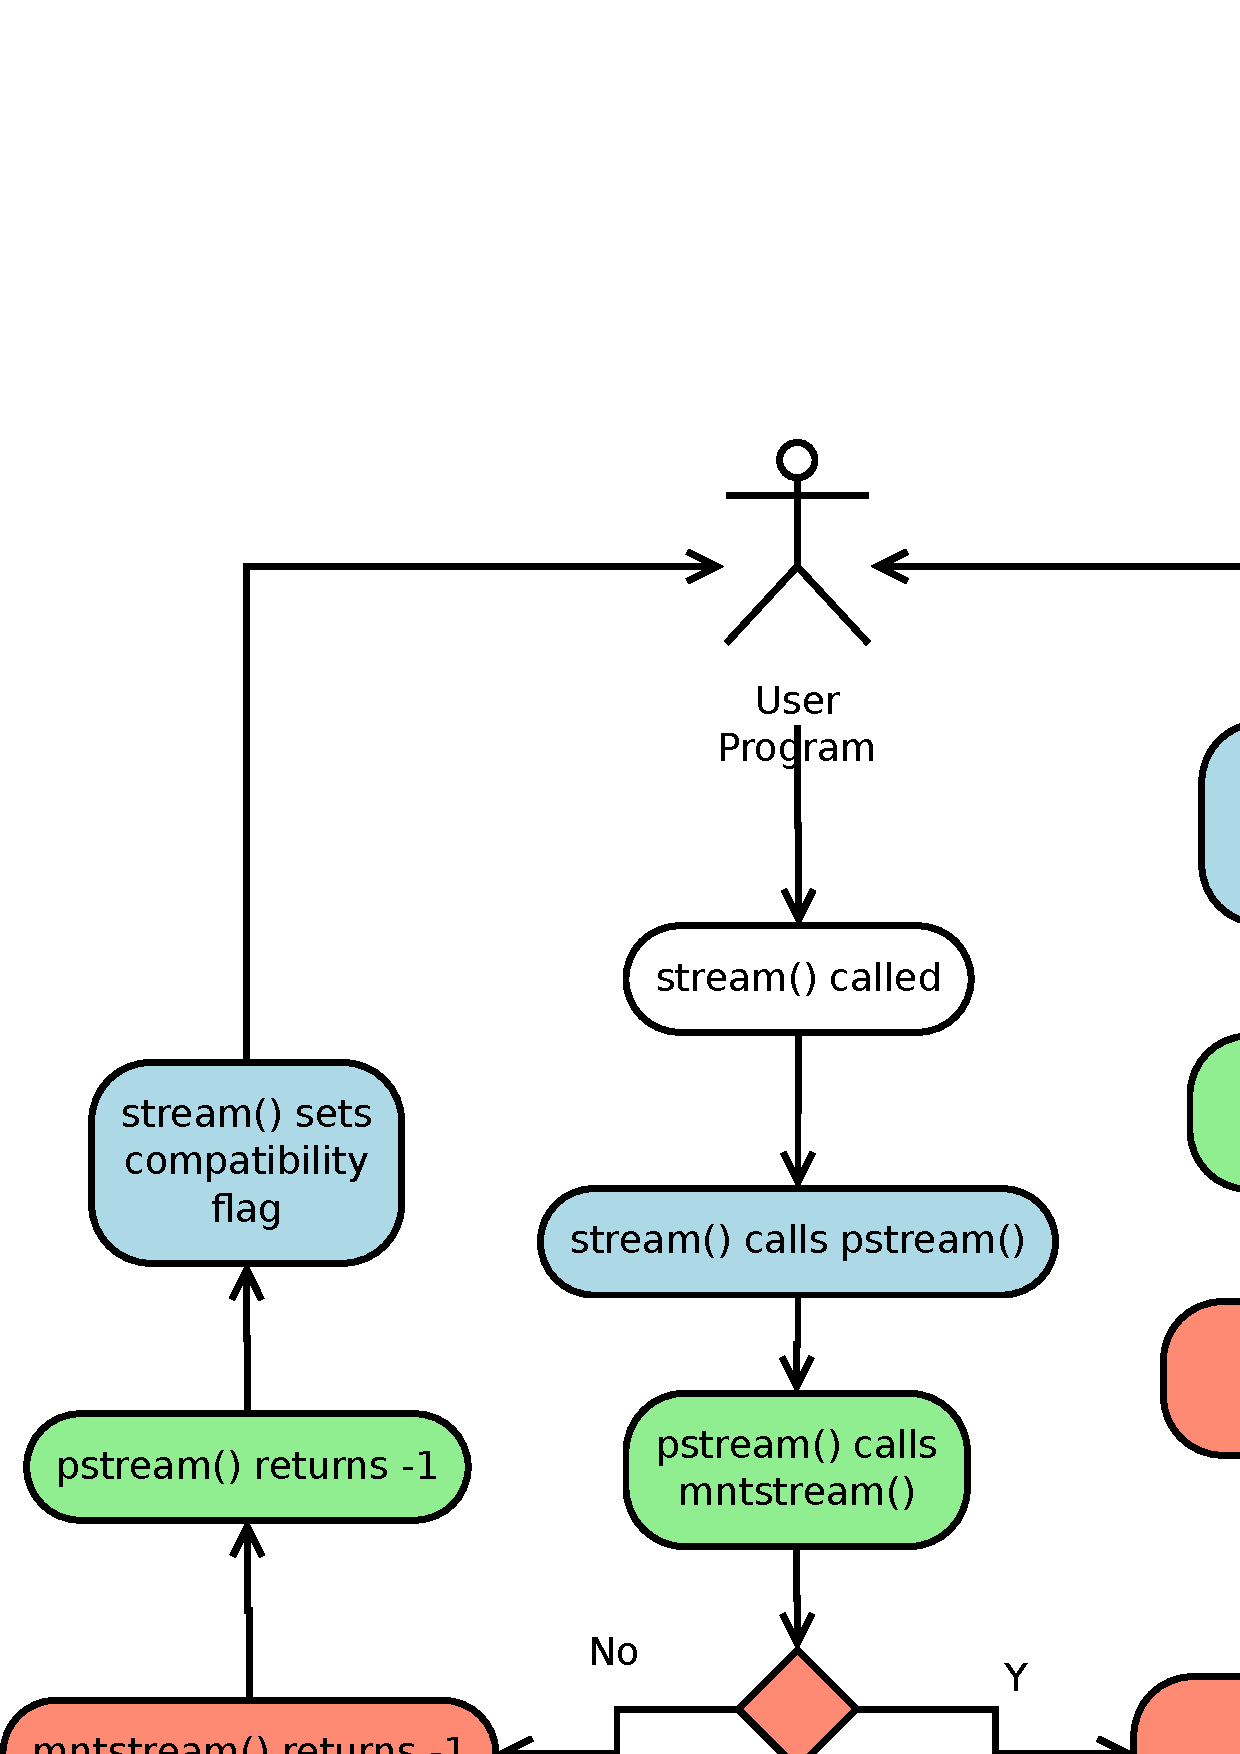
\includegraphics[width=0.85\textwidth]{flowchart.png}
\end{center}
\end{frame}

\section{Testing/Results}
\subsection{Test Programs}

\begin{frame}{Adapting Programs for Streaming}
\begin{itemize}
	\item It is simple to modify a user program to use streams
	\begin{itemize}
		\item Locate sequential file reading/writing situations
		\item After the file is opened, call {\tt stream} with the resulting file descriptor
		\item Call {\tt sread} or {\tt swrite} instead of {\tt read} or {\tt write}
	\end{itemize}
	\item 9P servers are slightly more difficult
	\begin{itemize}
		\item Have server report its version as 9P2000.s
		\item Add handler function for incoming {\tt Tstream} messages
		\item Begin listening on an open port
		\item Send {\tt Rstream} reply with IP and port
		\item Wait for connection
		\item Send/receive data to/from connection
	\end{itemize}
\end{itemize}
\end{frame}

\begin{frame}{The {\tt exportfs} file server}
\begin{itemize}
	\item The {\tt exportfs} file server was modified to serve streams
	\item {\tt exportfs} exports a server's namespace to a client
	\begin{itemize}
		\item Simple design
		\item Very commonly used
	\end{itemize}
	\item 9P message handler modified to recognize {\tt Tstream} messages
	\item If a stream is requested:
	\begin{itemize}
		\item {\tt exportfs} begins listening on an unused TCP port
		\item Sends back the IP address and port number in the {\tt Rstream} reply
		\item Waits until client connects to the port
		\item In the case of a read stream, continually send file data over the TCP connection until EOF.
		\item In the case of a write stream, continually read data over the TCP connection until no data remains.
	\end{itemize}
\end{itemize}
\end{frame}

\begin{frame}{Streaming {\tt cp}}
\begin{itemize}
	\item Standard {\tt cp} opens source and destination files, then copies 8 KB at a time using {\tt read} and {\tt write}
	\item In modified "streaming {\tt cp}", or {\tt scp}, both files are opened, then streams are created on the open files
	\item The source file is set up as a read stream
	\item Destination file is set up as a write stream
	\item {\tt sread} and {\tt swrite} are called to read 8 KB at a time from the read stream and write it back out to the write stream
	\item Compatibility mode allows use with non-streaming servers
	\item Modifications required the addition of 2 lines of code and slight changes to 2 other lines
\end{itemize}
\end{frame}

\begin{frame}{Testing Setup}
\begin{itemize}
	\item Used same setup as preliminary HTTP vs. 9P measurements
	\item Tests consisted of copying files over HTTP, streaming 9P, and non-streaming 9P
	\item As before, randomly-generated test files of 10MB, 50MB, 100MB, and 200MB were transferred
	\item Tests were performed with latencies of 500 $\mu$s, 15 ms, and 50 ms RTT
\end{itemize}
\end{frame}

\subsection{Results}

\begin{frame}{500 $\mu$s RTT}
\begin{center}
	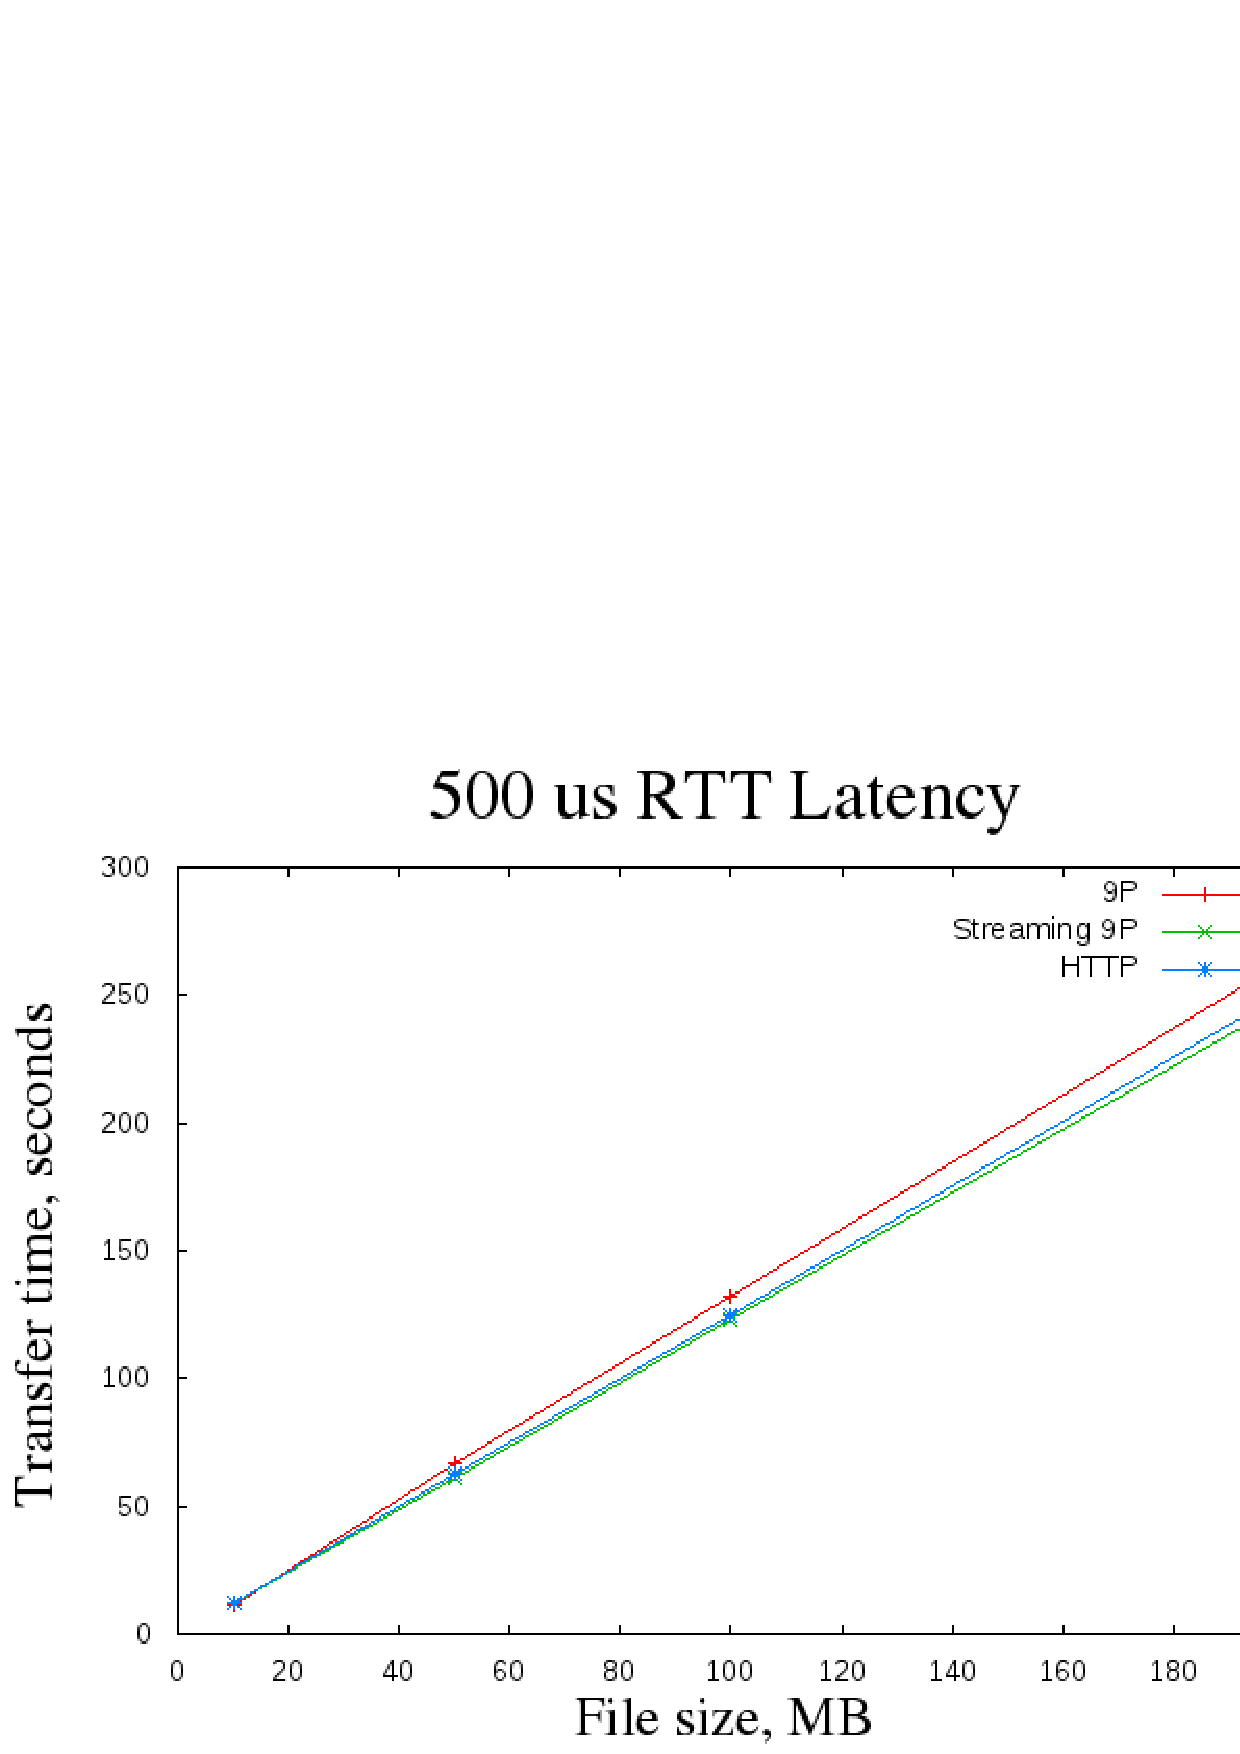
\includegraphics[width=0.65\textwidth]{results/500us-stream.png}
	\scriptsize{
	\begin{table}
		\begin{center}
			\begin{tabular}{ | c | c | c | c | }
			\hline
			\bf{File Size (MB)} & \bf{9P (sec.)} & \bf{Streaming 9P (sec.)} & \bf{HTTP (sec.)} \\ \hline
			10 & 11.36 & 12.21 & 12.56 \\ \hline
			50 & 67.23 & 61.29 & 62.41 \\ \hline
			100 & 132.34 & 123.32 & 124.49 \\ \hline
			200 & 263.33 & 247.34 & 251.22 \\ \hline
			\end{tabular}
		\end{center}
	\end{table}
	}
\end{center}
\end{frame}

\begin{frame}{15 ms RTT}
\begin{center}
	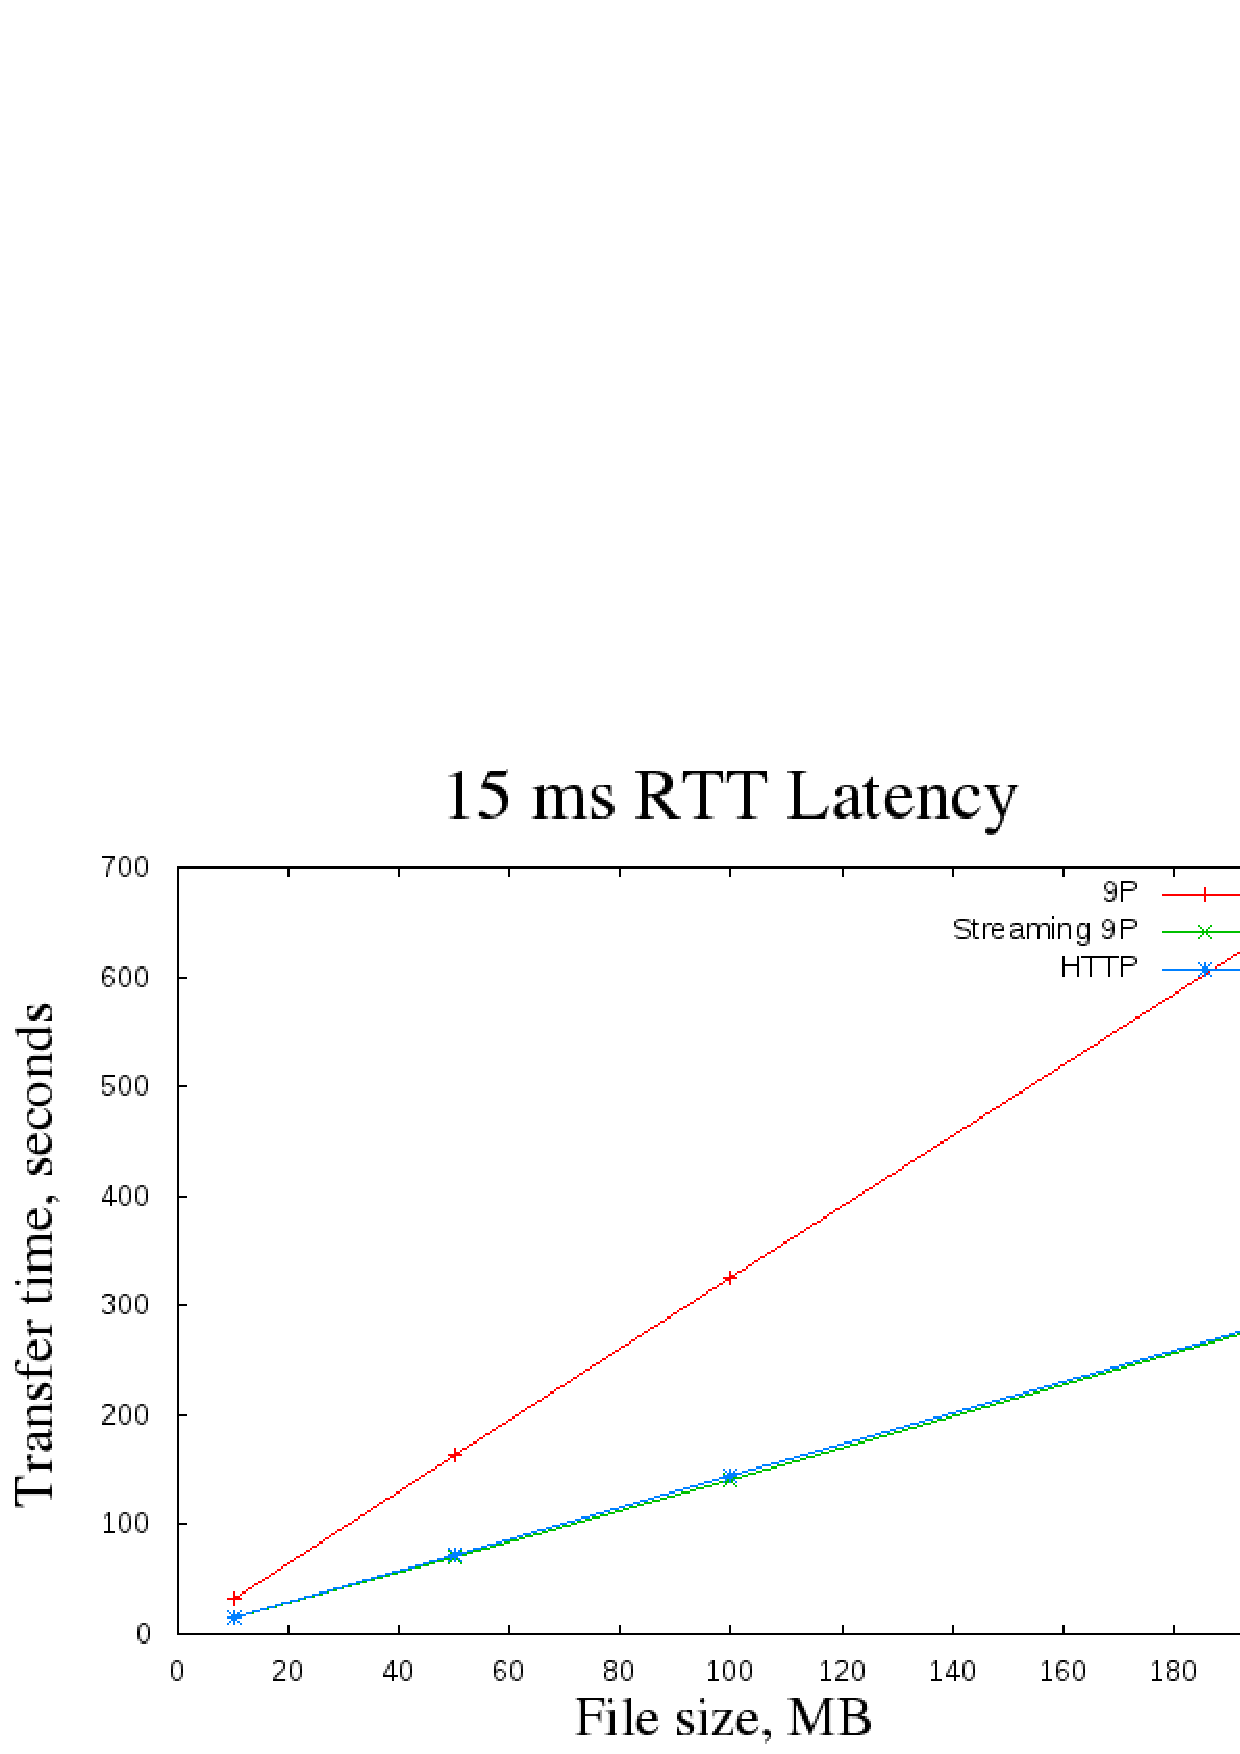
\includegraphics[width=0.65\textwidth]{results/15ms-stream.png}
	\scriptsize{
	\begin{table}
		\begin{center}
			\begin{tabular}{ | c | c | c | c | }
			\hline
			\bf{File Size (MB)} & \bf{9P (sec.)} & \bf{Streaming 9P (sec.)} & \bf{HTTP (sec.)} \\ \hline
			10 & 31.77 & 14.38 & 15.15 \\ \hline
			50 & 163.45 & 71.00 & 72.56 \\ \hline
			100 & 324.46 & 140.68 & 144.96 \\ \hline
			200 & 647.92 & 284.71 & 287.23 \\ \hline
			\end{tabular}
		\end{center}
	\end{table}
	}
\end{center}
\end{frame}

\begin{frame}{50 ms RTT}
\begin{center}
	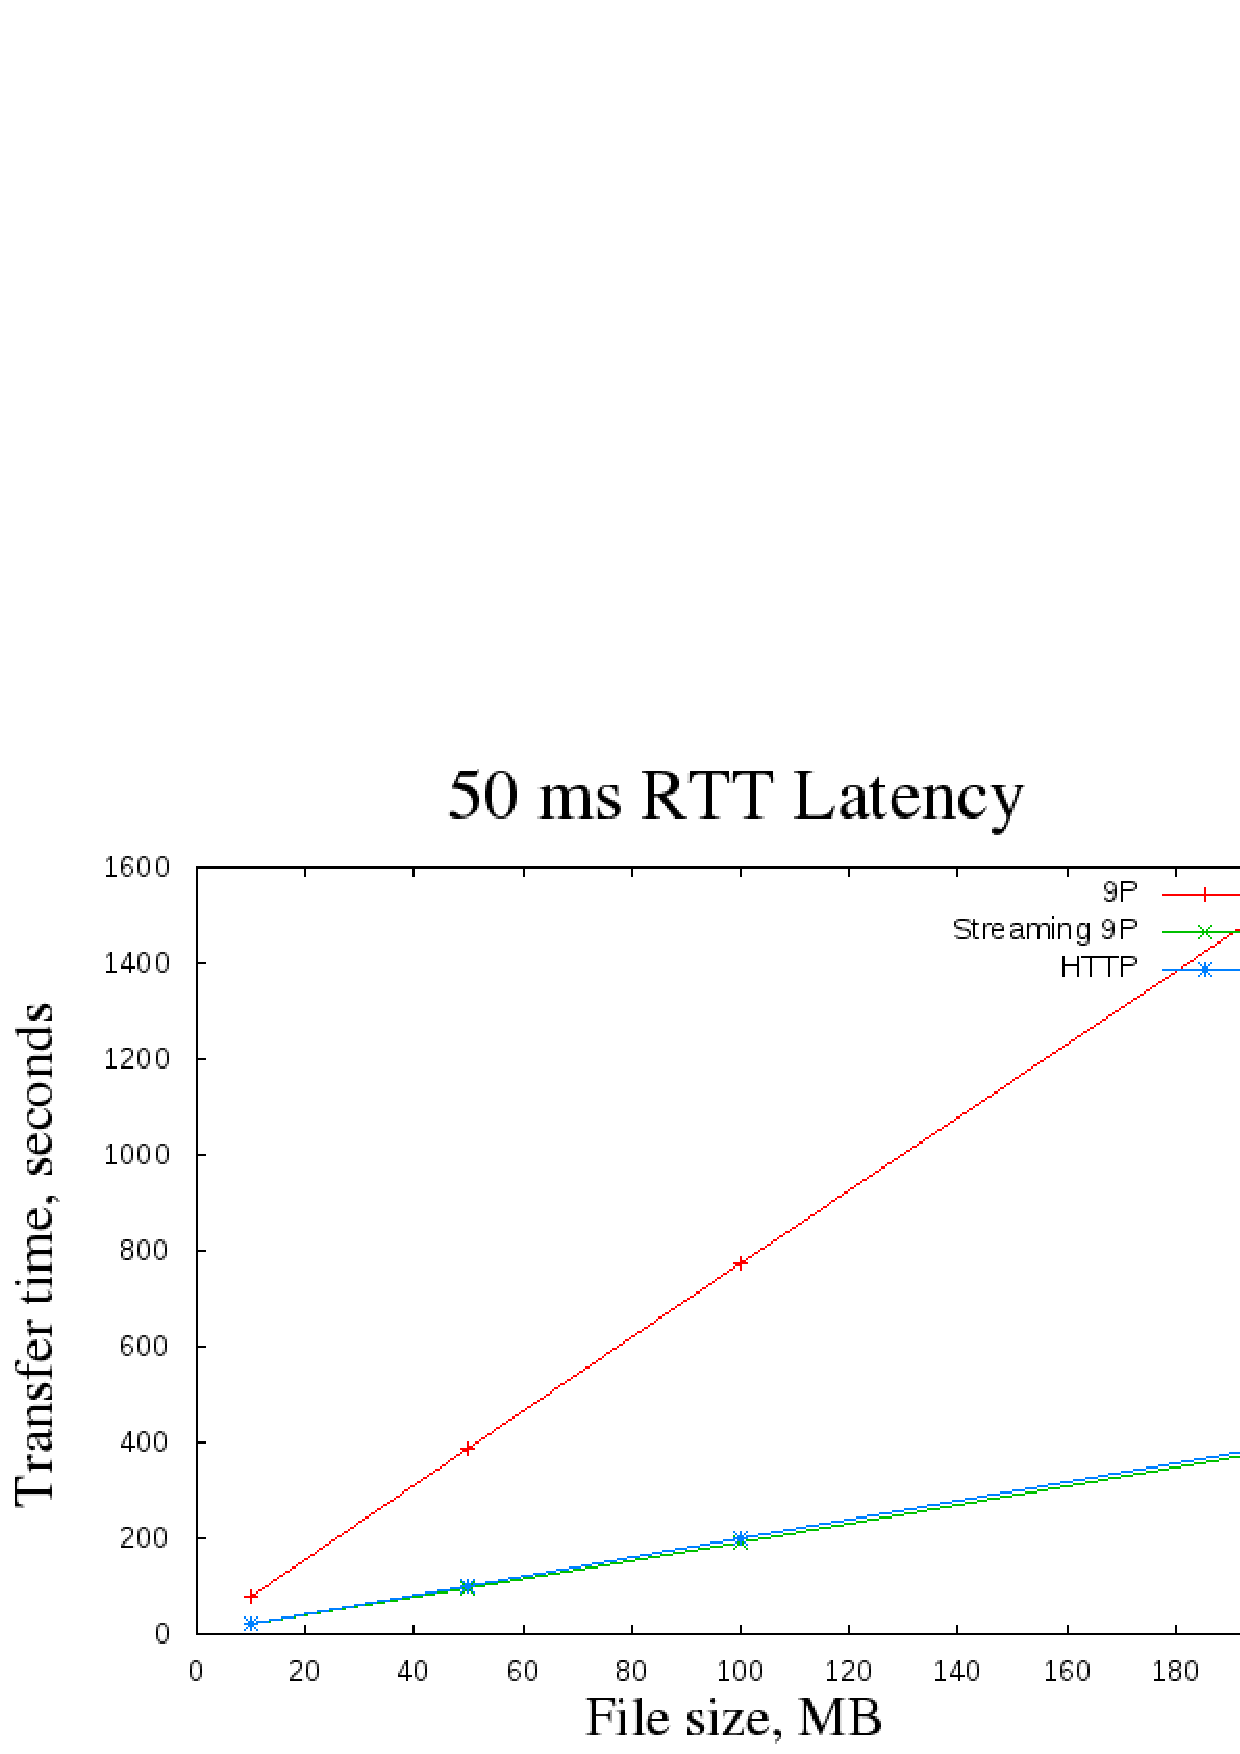
\includegraphics[width=0.65\textwidth]{results/50ms-stream.png}
	\scriptsize{
	\begin{table}
		\begin{center}
			\begin{tabular}{ | c | c | c | c | }
			\hline
			\bf{File Size (MB)} & \bf{9P (sec.)} & \bf{Streaming 9P (sec.)} & \bf{HTTP (sec.)} \\ \hline
			10 & 78.82 & 21.80 & 21.45 \\ \hline
			50 & 387.92 & 96.19 & 98.39 \\ \hline
			100 & 773.03 & 192.60 & 198.14 \\ \hline
			200 & 1535.81 & 385.69 & 395.53 \\ \hline
			\end{tabular}
		\end{center}
	\end{table}
	}
\end{center}
\end{frame}

\begin{frame}{Concurrent Downloads, 50 ms RTT}
\begin{center}
	\includegraphics[width=0.65\textwidth]{concurrent.png}
	\scriptsize{
	\begin{table}
		\begin{center}
		\begin{tabular}{ | c || c | c | c |}
			\hline
			\bf{Number of Clients} & \bf{Streaming 9P (sec.)} & \bf{HTTP (sec.)} & \bf{9P (sec.)} \\ \hline
			2 & 30.96 & 28.51 & 79.75 \\ \hline
			4 & 53.28 & 52.53 & 100.81 \\ \hline
			8 & 104.24 & 101.93 & 158.53 \\ \hline
		\end{tabular}
		\end{center}
	\end{table}
	}
\end{center}
\end{frame}

\section{Conclusions}

\begin{frame}{Future Work}
\begin{itemize}
	\item Other 9P servers, such as Fossil and Venti, should be converted to use streams
	\item User programs which can benefit from streaming should be modified:
	\begin{itemize}
		\item {\tt page} document and image viewer
		\item {\tt mp3dec} music player
	\end{itemize}
	\item Design may eventually be included in the Plan 9 distribution
\end{itemize}
\end{frame}

\begin{frame}{Conclusions}
\begin{itemize}
	\item Streaming 9P has demonstrated that it can match the performance of HTTP
	\item POSIX file semantics have been expanded to give attention to sequential file I/O
	\item Rather than try to improve performance transparently, explicit library functions let the programmer choose when streaming is important
	\item Requires very small programmer effort for large performance gains
\end{itemize}
\end{frame}

%\begin{frame}{Bibliography}
%%\bibliographystyle{plain}
%\bibliography{floren}
%\end{frame}
\setbeamertemplate{bibliography entry title}{}
\setbeamertemplate{bibliography entry location}{}
\setbeamertemplate{bibliography entry note}{}
\setbeamertemplate{bibliography item}{\insertbiblabel}
\begin{frame}[allowframebreaks]{Bibliography}
\bibliographystyle{plain}
\tiny{
        \bibliography{floren}
}
\end{frame}

\end{document}
